\documentclass[english,11pt,openany]{article}
\usepackage{graphicx}

\usepackage{subcaption}
\usepackage{ucs}
\usepackage[utf8]{inputenc}
\usepackage[executivepaper,margin=1in]{geometry}
%\usepackage[charter]{mathdesign}
\usepackage{babel}
% \usepackage{subfigure}
\usepackage{fancyhdr}
\usepackage{listings}
\usepackage{lmodern}
\usepackage{amsmath}
\usepackage{empheq}
\usepackage{amsthm}
\theoremstyle{definition}
\newtheorem{defn}{Definition}[section]
\newcommand{\E}{\mathbb{E}}
\newcommand{\R}{\mathbb{R}}
\newcommand{\bigO}{\mathcal{O}}
\usepackage[toc,page]{appendix}

\usepackage{booktabs}
\usepackage[svgnames,table]{xcolor}
\usepackage[tableposition=above]{caption}
\usepackage{pifont}

\theoremstyle{plain}
\newtheorem{Th}{Theorem}[section]
\newtheorem{Lemma}[Th]{Lemma}
\newtheorem{Cor}[Th]{Corollary}
\newtheorem{Prop}[Th]{Proposition}

\theoremstyle{definition}
\newtheorem{Def}[Th]{Definition}
\newtheorem{Conj}[Th]{Conjecture}
\newtheorem{Rem}[Th]{Remark}
\newtheorem{?}[Th]{Problem}
\newtheorem{Ex}[Th]{Example}

\newtheorem{theorem}{Theorem}
\usepackage{amssymb}
\usepackage[colorlinks=true]{hyperref} 
\hypersetup{urlcolor=blue,linkcolor=black,citecolor=black,colorlinks=true}
%\usepackage[usenames,dvipsnames,svgnames,table]{xcolor}
\definecolor{light-gray}{gray}{0.70}

\begin{document}

\begin{appendices}
	
\subsection{Complexity}

Let us consider p predictor variables $(x_1, \cdots, x_p) \in D \subset \R^p$  of a response variable $y$. The goal of this subsection is to determine the time complexity of the Random Forest model, given $N$ samples data. 
\newline
Let $T(N)$ denote the time for building one decision tree. 

\begin{figure}[h!]
	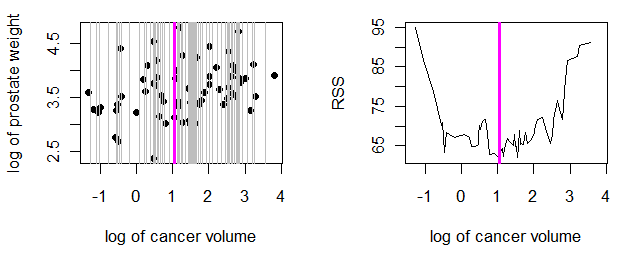
\includegraphics[scale=0.8]{sorting_split.png}
	\caption{Choosing the best vertical split using RSS measure} \label{figure:sorting}
\end{figure}


$T(N)$ can be approximated recursively. 
Indeed, we can grow a decision tree in three steps : find the best splitting, grow a left child tree, and grow a right child tree.
\newline 
Let us denote the time complexity of these steps by $s(N)$, $T_{left}(N)$ and $T_{right}(N)$ respectively. 
Hence : $T(N) = s(N) + T_{left}(N) + T_{right}(N)$.
We will present both best case and worst case complexity for every step, and we will assume the time complexity to lay in between. 
\paragraph{splitting and partitioning}
	The partitioning step requires at least an iteration over the N samples, so we can already set a linear lower bound on the time complexity within a node.
	Finding a split can be done using Figure \ref{figure:sorting} (example from \cite{Cutler:slides}) method, i.e computing a Residual Sum of Squares (RSS) and minimize it. 
	This operation requires to sort the N samples for every predictor $x_i, i\in \{1, \cdots, p\}$. 
	Time complexity to sort a list with size $N$ is at worst $\mathcal{O} (N)$, and at best $\bigO(\log N)$. 
	Combining both splitting and partitioning, time complexity is at worst $\mathcal{O} (p N^2)$ and at best $\bigO(p N \log N)$ . 
	Random Forest can limit the search over $K \leq p$ features, which reduces this complexity between $\mathcal{O} (K N\log N)$ and $\mathcal{O} (K N^2)$. 
	
\paragraph{Child left and right trees}

The best case for growing these two child trees is intuitively $\frac{N}{2}$. The worst case would be having a tree with one pure leaf	and $N - 1$ samples in the other tree. 

Hence, 
\begin{displaymath}
s(N) + T_{left}(\frac{N}{2}) + T_{right}(\frac{N}{2}) \leq T(N) \leq s(N) + T_{left}(1) + T_{right}(N - 1) 
\end{displaymath}
Or

\begin{displaymath}
s(N) + 2.T(\frac{N}{2})\leq T(N) \leq s(N) + T(1) + T(N - 1) 
\end{displaymath}

 
Having a recurrence equation, let us make use of the following theorem. 

\begin{Th}\label{theorem:master}Master Theorem
	
	$$T(n) = \left\{ \begin{array}{ll}
	c             & \mbox{if $n < d$,}\\
	aT(n/b) + f(n)& \mbox{if $n \geq d$},
	\end{array}
	\right. $$
	where $a \geq 1, b > 1,$ and $d$ are integers and $c$ is a positive
	constant.  Let $\nu = \log_b a$.
	\begin{description}
		\item[Case (i) $f(n)$ is ``definitely smaller'' than $n^\nu$:] If there is a small contant $\epsilon > 0,$ such that 
		$f(n) \preceq n^{\nu - \epsilon}$, that is,
		$f(n) \prec n^\nu$, then $T(n) \sim n^\nu$.
		
		\item[Case (ii) $f(n)$ is ``similar in size'' to $n^\nu$:] If there is a constant $k \geq 0$, such that 
		$f(n) \sim n^{\nu}( \log n)^k$, then 
		$T(n) \sim n^{\nu}(\log n)^{k+1}$.
		
		\item[Case (iii) $f(n)$ is ``definitely larger'' than $n^\nu$:] If there are small constants $\epsilon > 0$ and $\delta < 1$, such
		that $f(n) \succeq n^{\nu + \epsilon}$ and $a f(n/b) \leq \delta
		f(n),$ for $n \geq d$, then $T(n) \sim f(n)$.
		
	\end{description}
\end{Th}

\vspace{0.5cm}
\begin{Lemma}
	For $\frac{s(N)}{K} = \mathcal{O} (N\log N)$ and $T(N) = 2.T(\frac{N}{2}) + s(N)$, 
	time complexity for building a decision tree is $T(N) \sim K.N.\log^2N$.
\end{Lemma}

\begin{proof}
	Apply Theorem \ref{theorem:master} with $a=b=2$, $d=1$, $k=1$ and $T(N) \equiv \frac{T(N)}{K}$
\end{proof}


\begin{Lemma}
	For $\frac{s(N)}{K} = \mathcal{O} (N\log N)$ and $T(N) = s(N) + T(1) + T(N - 1) $, time complexity for building a decision tree is $T(N) \sim K.N.\log^2N$ (upper bound) and $T(N) $.
\end{Lemma}

\begin{proof}
	Let us rewrite in a first time the expression of $T(N)$ in a better form to make use of Theorem \ref{theorem:master}. 
	
	\begin{displaymath}
	\frac{s(N)}{K} = \mathcal{O} (N\log N)
	\end{displaymath}
	
	Let us assume there exists $C_1$, $C_2$ such that $C_1 N\log N \leq \frac{s(N)}{K} \leq C_2 N\log N$. 
	Hence, using the right side, 
	
	\begin{align}
	\frac{T(N)}{K}	& = \frac{s(N)}{K} + \frac{T(1)}{K} + \frac{T(N - 1)}{K} \notag \\
					& \leq C_2 N\log N + \frac{T(1)}{K} + \frac{T(N - 1)}{K}\notag
	\end{align}
	
	Let $t(N) = \frac{T(N)}{K}$. 
	
	\begin{align}
	& t(N) \leq C_2 N\log N + t(1) + t(N-1)\notag \\
	\iff &  t(N) - t(N-1) \leq C_2 N\log N + t(1) \notag\\
	\Rightarrow & \sum_{j=2}^{N}  t(j) - t(j-1) \leq (N-1)t(1) + C_2\sum_{j=2}^{N}j \log j \notag\\
	\Rightarrow & t(N) \leq Nt(1) + C_2\log N \sum_{j=1}^{N}j \notag\\
	\Rightarrow & t(N) \leq Nt(1) + C_2\log N \frac{N(N +1)}{2}\notag \\
	\Rightarrow & t(N) = \bigO (N^2 \log N) \notag \\
	\Rightarrow & T(N) = \bigO (KN^2 \log N) \notag
	\end{align}
	
	Similarly, using the left side gives a lower bound 
	
	\begin{align}
	& t(N) \geq C_1 N\log N + t(1) + t(N-1)\notag \\
	\iff &  t(N) - t(N-1) \geq C_1 N\log N + t(1) \notag\\
	\Rightarrow & \sum_{j=2}^{N}  t(j) - t(j-1) \geq (N-1)t(1) + C_1\sum_{j=2}^{N}j \log j \notag\\
	\Rightarrow & t(N) \geq N t(1) + C_1 \sum_{j=2}^{N}j \notag\\
	\Rightarrow & t(N) \geq Nt(1) + C_1 (\frac{N(N +1)}{2} - 1)\notag \\
	\Rightarrow & t(N) \succeq N^2 \notag \\
	\Rightarrow & T(N) \succeq N^2 \notag
	\end{align}
	
\end{proof}

Finally, growing $n_{trees}$ random trees has in the best case a time complexity $\Theta(n_{trees}KN\log^2 N)$ and in the worst case $\bigO (n_{trees} K N^2 \log N)$.

\paragraph{Prediction time complexity}

Iterating over every tree generated by the Random Forest, predicting depends on the depth of the tree. 
Similarly to previous analysis, we can lower bound and upper bound the depth of one tree. 
Indeed, let $D(N)$ denote the depth of a tree generated in the Forest. 

\begin{itemize}
	\item 
	Best case is again a $\frac{N_{at\_node\_i}}{2}$ split at every node $i$,  which gives the following recurrence equation for prediction: 
	\begin{align}
	\begin{cases}
	D(1) = 1 \\
	D(N) = 1 + D(\frac{N}{2}) + D(\frac{N}{2}) = 1 + 2.D(\frac{N}{2})
	\end{cases}
	\end{align}
	
	A quick application of Theorem \ref{theorem:master} with $a=b=2$ and $k=0$ gives $D(N)\sim \log N$
	
	\item Worst case is a split with one simple leaf and a tree with $N-1$ samples, which gives the following recurrence equation : 
	\begin{align}
	\begin{cases}
	D(1) = 1 \\
	D(N) = 1 + D(1) + D(N-1) \notag
	\end{cases}
	\end{align}
	
	\begin{align}
	D(N) - D(N-1) & = 1 + D(1) \notag \\
	D(N) &= (N + 1)D(1) \notag \\
	D(N) & = \bigO(N) \notag 
	\end{align}
	 
\end{itemize}


\end{appendices}

\end{document}